\section{Research Methodology}

% NEED TO REWRITE THIS SECTION

\subsection{Experimental Design}
For my experimental design, a participant was shown 5 pairs of room layouts in the form of a 2 Staged A/B test.
In the first stage the participant was informed to pick, out of each pair, which room furniture layout they preferred. This preference may have been influenced by realism, authenticity or what environment they would rather be in. In each pair, one layout was that of human design and the other was designed by the Artefact (M-A System) - an example of this is shown in Fig~\ref{pair-example-1} \& Fig~\ref{pair-example-2}. The order in which these layouts were shown were randomised per stage and per participant.
Once 5 furniture arrangements were selected, the participant would move onto the second stage of the study - a notice would appear notifying the participant they have reached Stage 2, as shown in Fig~\ref{stage-2}. Just before beginning they were notified that in every pair within the first stage, 1 furniture layout was created by the Artefact (M-A System). Their challenge in the second stage of the study would be to select, out of the same 5 pairs they were initially shown, which one they believe was made by the Artefact (M-A System).

This experimental design was used as previous works by \italic{P. Henderson, et al.} \cite{constrained-layouts} and \italic{L.-F. Yu et al.} \cite{make-it-home} carried out similar perceptual studies requiring a participant to pick between one from their designed model and human designs. In 2010, Margaret Boden proposed a new variant of the Turing Test (TT) that is oriented around artistic creativity \cite{artistic-tt}. With her TT, for an art program to pass it would have to:
\begin{enumerate}
    \item Be indistinguishable from human produced artwork
    \item[]And/Or
    \item Be seen having similar aesthetic value to human produced artwork
\end{enumerate}
I found this variant of the TT as a helpful source when designing the experimental design for my research study.


\begin{figure}[!h]
    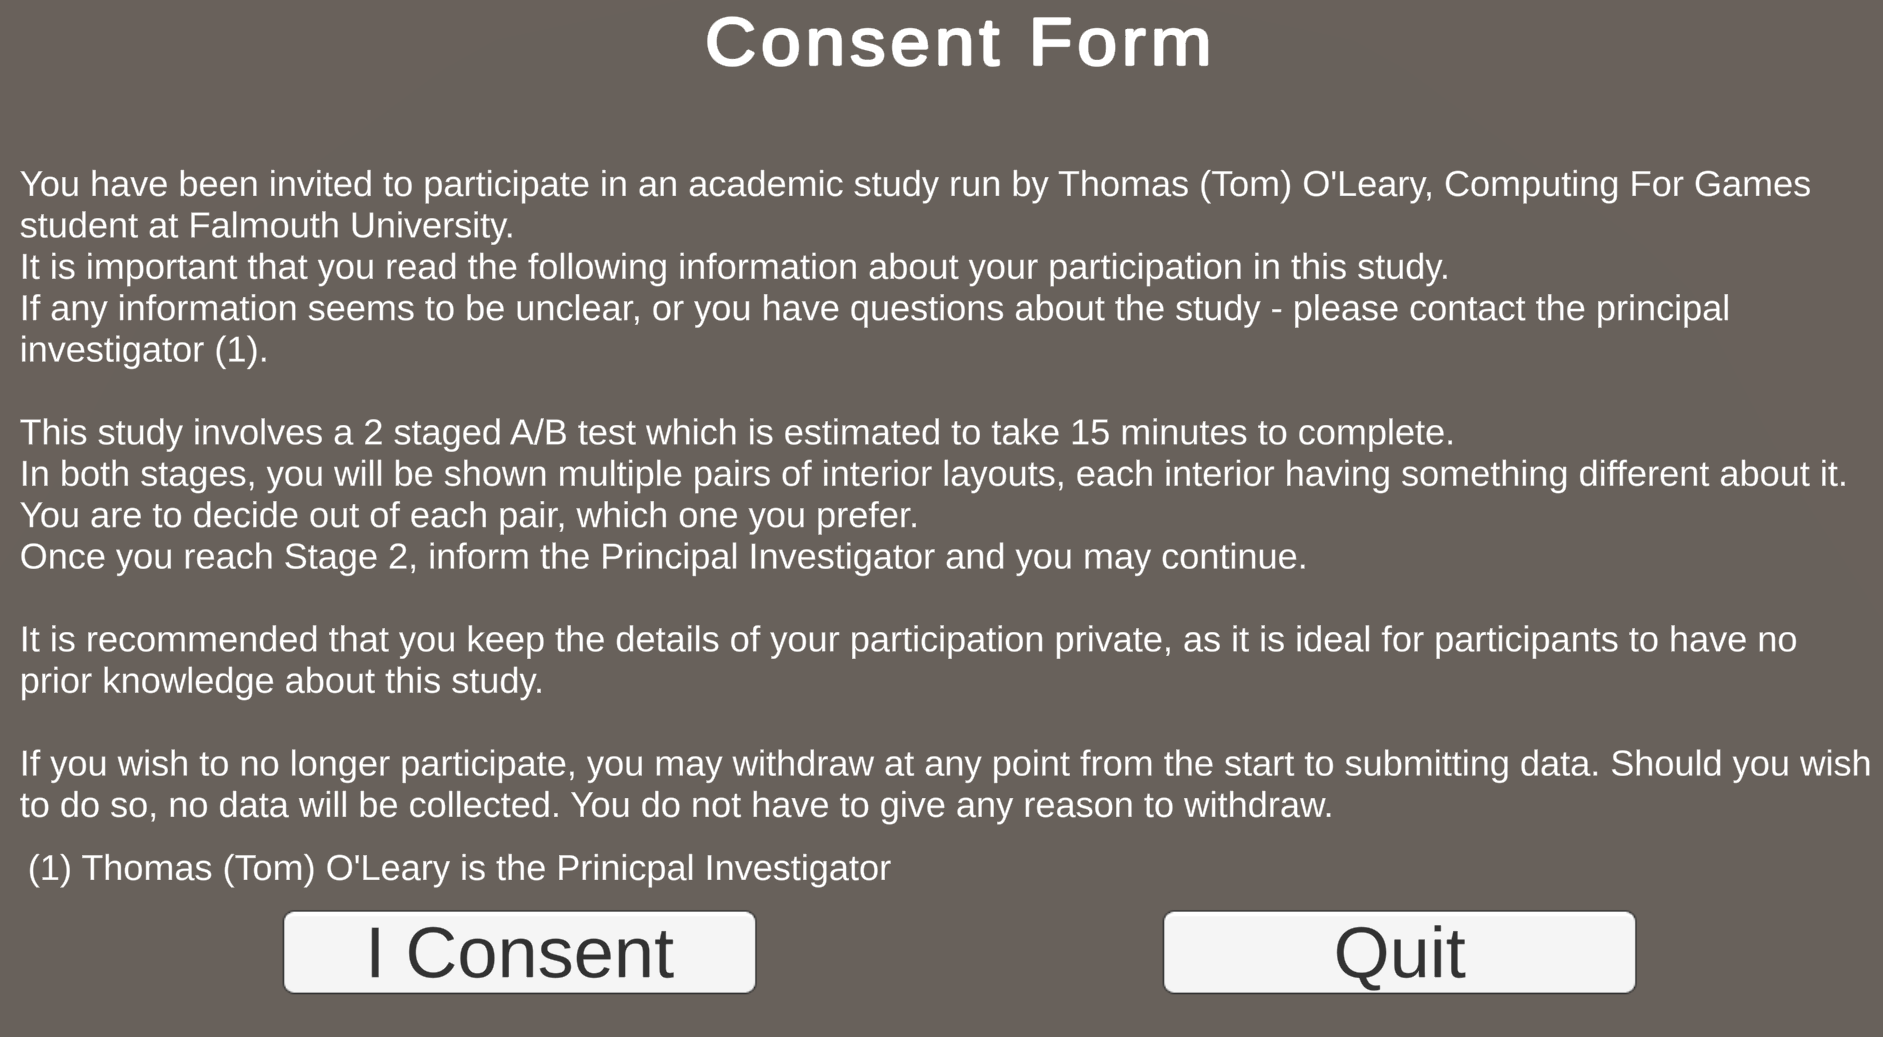
\includegraphics[width=\columnwidth]{./Images/consent-form.png}
    \centering
    \caption{The consent page before the start of the A/B test that the participant reads.}
    \label{consent-screen}
\end{figure}
\begin{figure}[!h]
    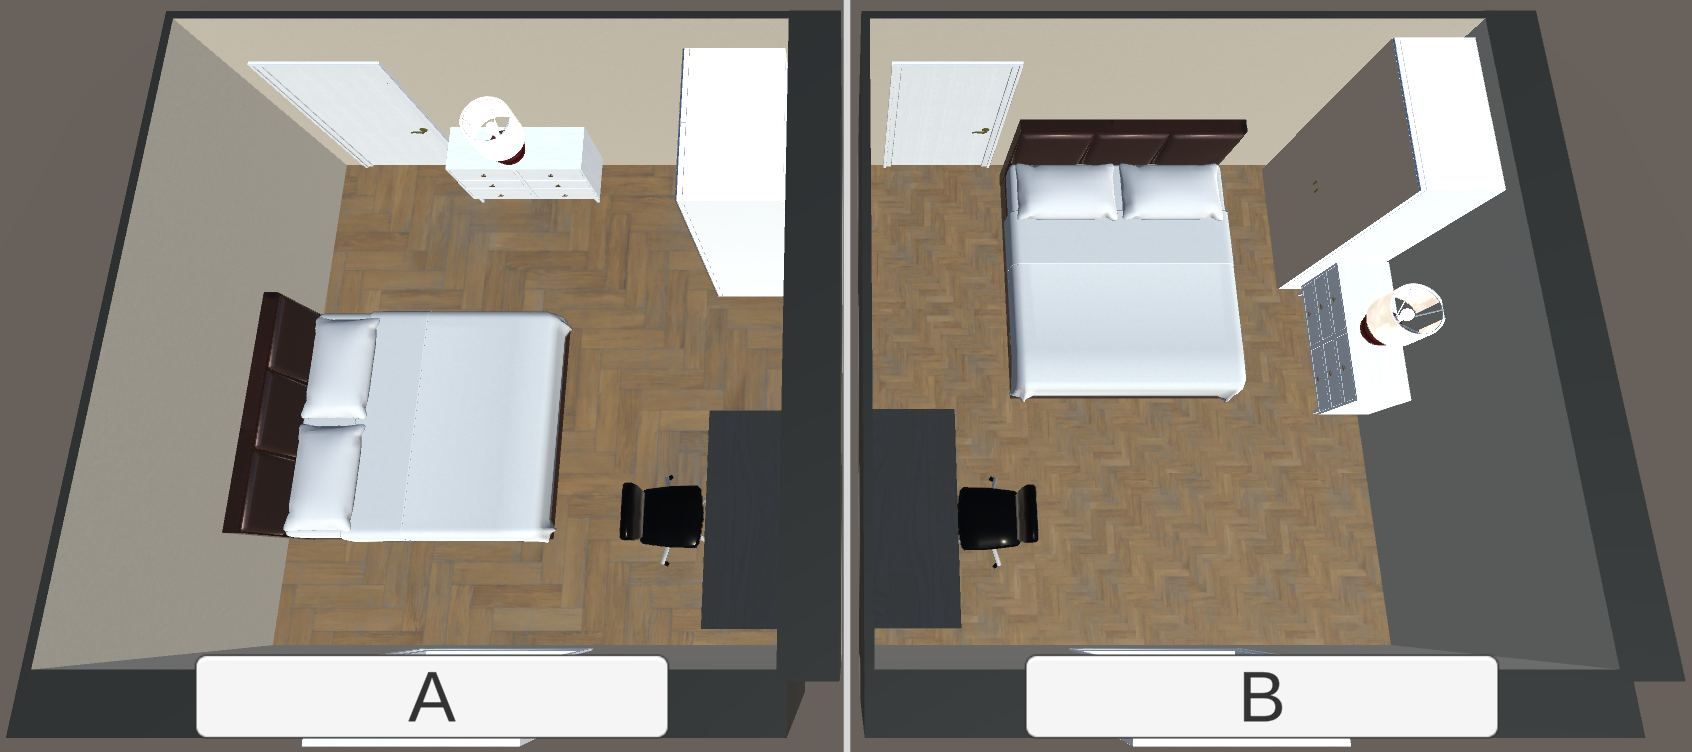
\includegraphics[width=\columnwidth]{./Images/pair-3.png}
    \centering
    \caption{A pair of furniture layouts used in the Research Study. One being human designed and the other being Artefact designed.}
    \label{pair-example-1}
\end{figure}
\begin{figure}[!h]
    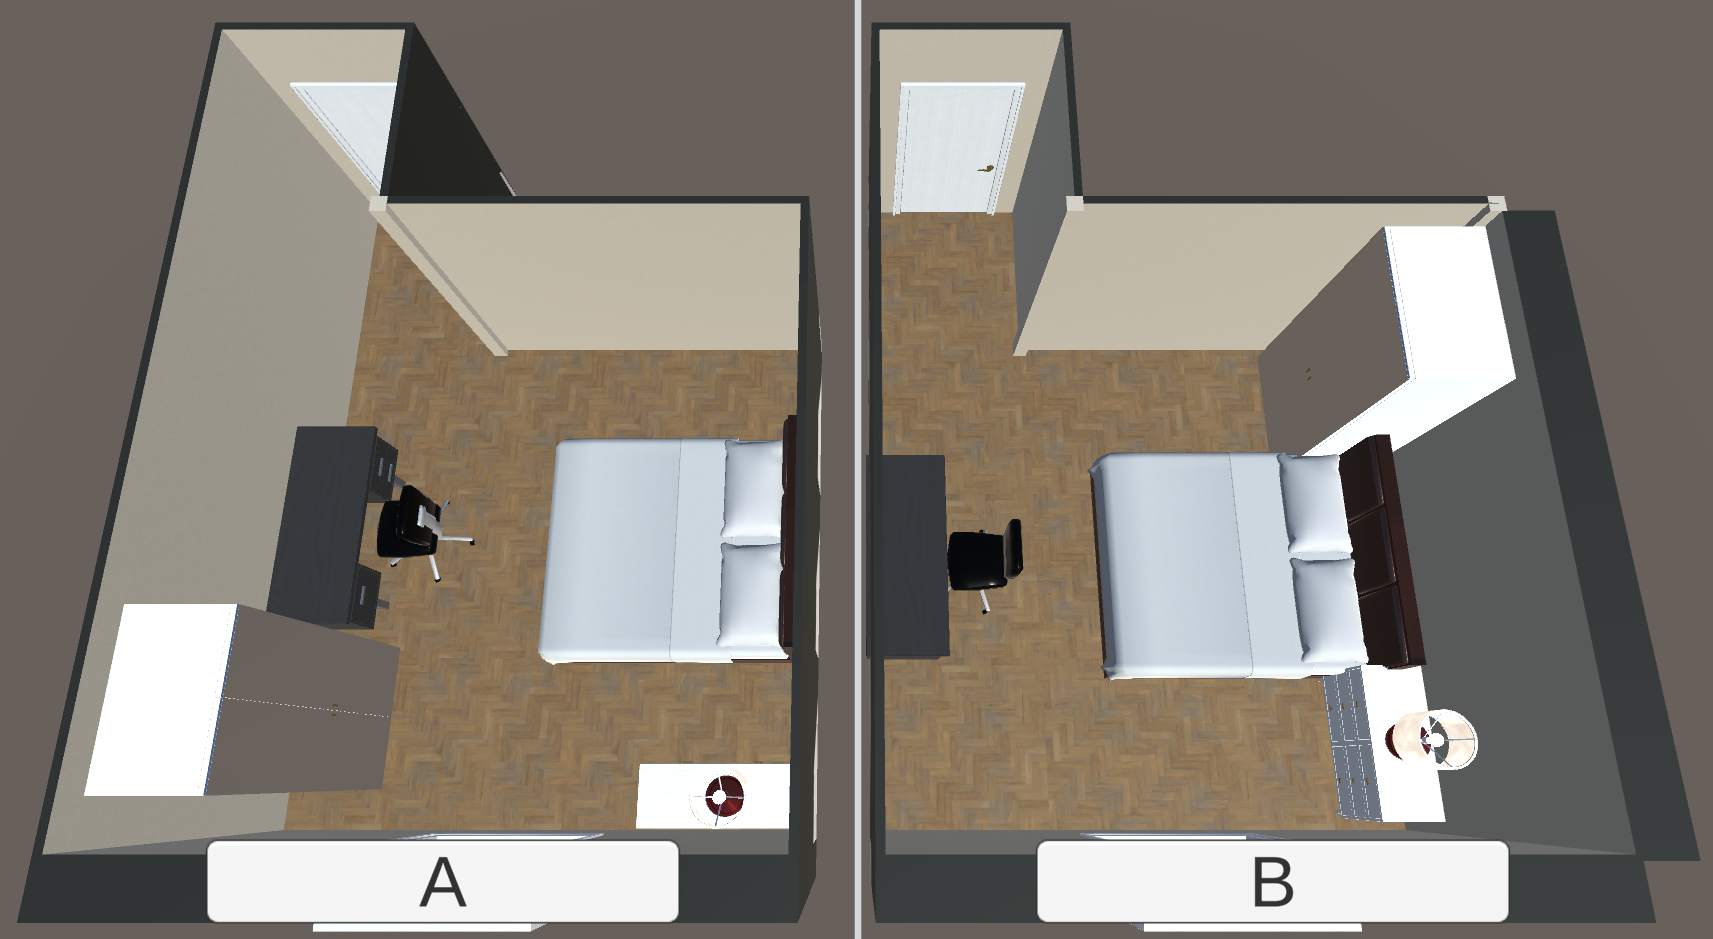
\includegraphics[width=\columnwidth]{./Images/pair-1.png}
    \centering
    \caption{Another pair that is used in the Research Study.}
    \label{pair-example-2}
\end{figure}
\begin{figure}[!h]
    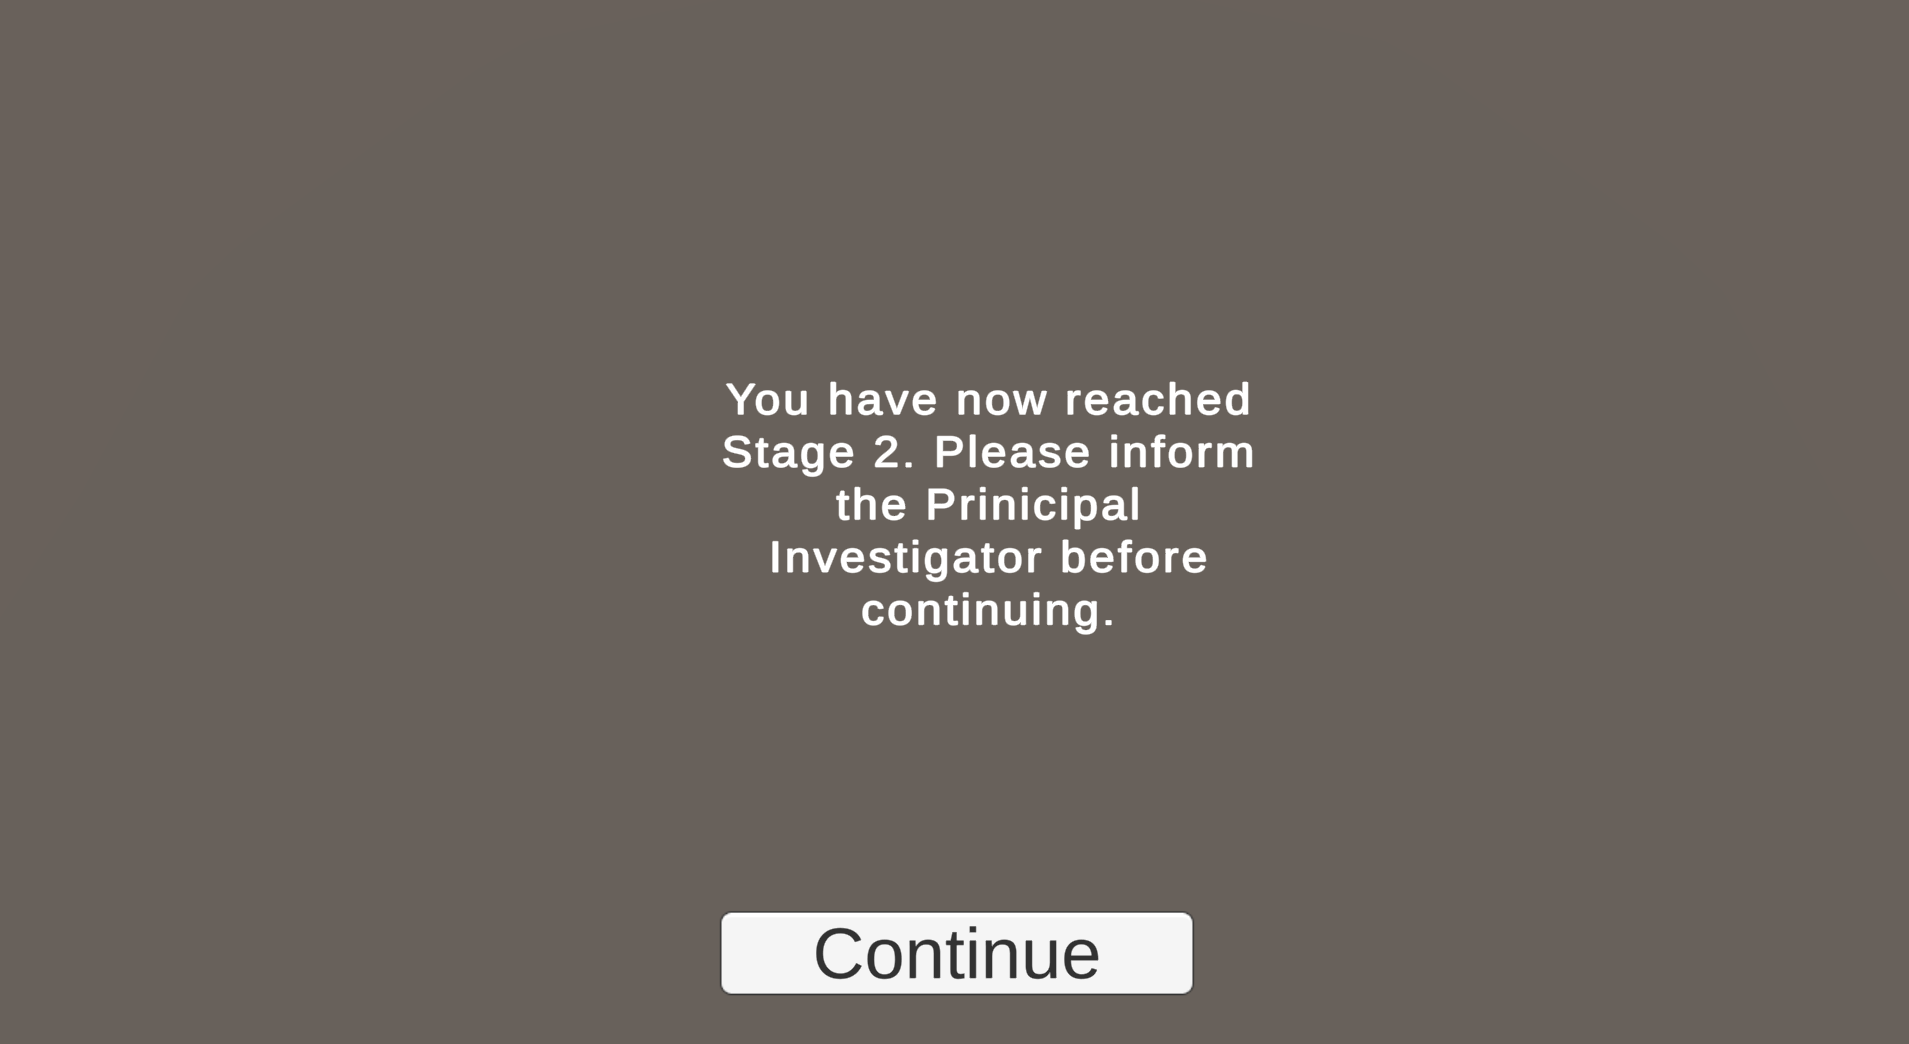
\includegraphics[width=\columnwidth]{./Images/stage-2-notice.png}
    \centering
    \caption{Screenshot of the Stage 2 notice, where participants are notified of the involvement of the Artefact.}
    \label{stage-2}
\end{figure}


\subsection{Sampling Plan}
To help answer my Hypotheses, I will be using two tailed T-Tests to allow me to easily identify the relationship between the selection of Human and Artefact designed layouts.
Using G*Power \cite{gpower}, I was able to calculate a sample size of 54 with an effect size of 0.5 - see Fig~\ref{gpower}.

\subsection{Data management plan}
As explained in Section \hyperref[ethics]{E}, no personal information is collected in the research study, nor can any information collected in the research study can be used to identify participants - signifying that General Data Protection Regulation (GDPR) \cite{gdpr} does not need to be followed. Results collected from the study however were exported and stored in a CSV file - see Fig~\ref{csv-file}. This file was password encrypted to prevent any third party intervention.


\subsection{Data Analysis}
Once sufficient data was collected from the research study, I used the R language and R-Studio for my analysis. In the code sample listed in \hyperref[append:b]{Appendix B}, I have demonstrated how to complete a Two Tailed T-Test using data from an imported CSV file.

\subsection{Ethical Considerations}\label{ethics}
As the research study requires human participants this creates a medium ethics risk according to the Falmouth University Ethics Board. To facilitate this risk, a Falmouth University ethics form was completed and signed off by the project Supervisor in consultation with the Head of Subject. The artefact itself is of low risk/concern as it is not used for militarization and participants are able to opt out at any point during their participation.
No personal information about the participants involved is collected nor can any data collected in the research study be used to identify participants - the EU's General Data Protection Regulation (GDPR)\cite{gdpr} does not need to be followed due to the nature of the research study. However, to protect the participants rights, the Nuremberg Code will be followed to keep and ensure this research study is ethically sound\cite{nuremberg-code}. All participants will be handed a Participant Information Sheet that details the key information they must know before the study, a consent form is also supplied to ensure they have agreed to participate. Participants are still able to withdraw at any point until submitting data.
\\
\subsubsection*{COVID-19}
At the current state of the pandemic and following the latest Government Guidelines in England \cite{gov-guidlines}, participants were not required to wear a face covering however they would not be questioned if they preferred to do so. All surfaces were sanitised between participants.
\\
\subsubsection*{Computer Related Injuries}
Due to the nature of the study taking place on a Computer, all forms of computer related injuries were taken into account. Participants had the opportunity to appropriately set the computers screen and seat positioning to the best ergonomic setting for themselves before starting the study. Participants were also informed that they could take a short break whenever they pleased.